\chapter{Grafi Multi-livello}\label{cap:grafi-multi-livello}

Come si \`e potuto vedere dal contenuto del Capitolo~\ref{cap:grafi-e-approccio-multi-livello},
le operazioni di contrazione e la costruzione di
gerarchie di grafi a pi\`u livelli siano concetti gi\`a ampiamente utilizzati e consolidati nella teoria dei grafi e
nelle sue applicazioni.
Tuttavia, ci\`o che non \`e stato ancora propriamente considerato nella letteratura esistente \`e la possibilit\`a di
definire e formalizzare una vera e propria struttura dati astratta che rappresenti un grafo multi-livello come
un'entit\`a a s\`e stante.
In questo capitolo verranno date le fondamenta per la definizione del concetto di \textit{Grafo Multi-livello} dal
punto di vista algebrico, e verranno introdotte le operazioni di base che permetteranno di rendere
algoritmicamente realizzabile la costruzione di tale struttura dati.

\section{Definizioni e propriet\`a di base}\label{sec:definizioni-e-proprieta-di-base}

In questa sezione saranno proposte definizioni e propriet\`a di base di una struttura dati per la rappresentazione
di gerarchie di grafi a pi\`u livelli, in cui sia possibile ottenere informazioni sull'intera struttura gerarchica in
relazione ai singoli grafi che la compongono, come attraverso l'espansione e la contrazione di nodi.
In particolare, riprendendo dalla terminologia e dai concetti esistenti in letteratura, si proporranno definizioni
originali di \textit{grafo decontraibile} e di \textit{grafo multi-livello}.

\subsection{Grafo decontraibile}

A partire dal concetto noto di grafo quoziente e di contrazione, si vuole definire una particolare
tipologia di grafi quoziente che, oltre a rappresentare le caratteristiche strutturali ad alto livello di astrazione
dei grafi da cui sono derivati, siano in grado di mantenere l'informazione originale di questi ultimi, in
che modo essa sia legata alla sua rappresentazione astratta. \newline
Nasce così il concetto di grafo decontraibile, che intuitivamente pu\`o essere considerato come un grafo
in cui i nodi sono riconducibili ad un grafo e gli archi ad un insieme di archi tra i nodi dei grafi
associati ai nodi coinvolti.
\newpage

\begin{definition}[Grafo decontraibile]
    Un \textbf{grafo decontraibile} $G$ \`e una quadrupla $(V, E, dec_V, dec_E)$ dove:
    \begin{itemize}
        \item $V$ \`e un insieme di elementi detti \textbf{supernodi};
        \item $E \subseteq V \times V$ \`e un insieme di coppie ordinate di supernodi, dette \textbf{superarchi};
        \item $dec_V : V \rightarrow \mathcal{G}_D$ \`e una funzione tale per cui $dec_V(v) = (\mathcal{V}_v,
            \mathcal{E}_v, dec_{\mathcal{V}_v}, dec_{\mathcal{E}_v})$ \`e un grafo decontraibile rappresentato
            dal supernodo $v$;
        \item $dec_E : E \rightarrow (\mathcal{V} \times \mathcal{V})$ con $\mathcal{V} = \bigcup_{v \in V}\mathcal{V}_v$,
            \`e una funzione tale per cui $\forall$ $ e = (u, v)$, \\ $dec_E(e) = \mathcal{E}_e \subseteq$ $\{(a, b)$ $\mid$ $a \in \mathcal{V}_u$ $\wedge$
            $b \in \mathcal{V}_v\}$ \`e un insieme di archi rappresentati dal superarco $e$.
    \end{itemize}
\end{definition}

Nella definizione, cos\`{i} come d'ora in avanti, si utilizzer\`a la notazione $\mathcal{G}_D$ per indicare l'insieme
dei grafi decontraibili, e le notazioni $\mathcal{V}$ e $\mathcal{E}$ per
indicare, rispettivamente, insiemi di supernodi e superarchi ottenibili attraverso decontrazioni e, quindi, di
livello inferiore rispetto al grafo decontratto di riferimento.
Le notazioni $\mathcal{V}_v$ e $\mathcal{E}_v$ saranno utilizzate per indicare, rispettivamente,
insiemi di nodi e archi di grafi ottenibili attraverso la decontrazione di un certo supernodo $v$.
Nel contesto di un determinato grafo decontraibile, per portare maggiore distinzione si continuer\`a ad utilizzare
il termine di nodo ed arco per riferirsi ai supernodi e superarchi di tale livello inferiore. \newline

Si noti che \`e possibile usare una notazione basata su attributi, alternativa a quella delle funzioni, per
descrivere le propriet\`a caratteristiche di nodi ed archi che rendono tale un grafo decontraibile.
Tale notazione sar\`a utilizzata in seguito per semplificare la descrizione di algoritmi. \newline
In particolare, si pu\`o definire un grafo decontraibile come un normale grafo diretto sotto forma di coppia
$(V, E)$ dove:
\begin{itemize}
    \item $\forall$ $v \in V,$ \`e definito un attributo $v.dec = G_v$ dove $G_v = (\mathcal{V}_v, \mathcal{E}_v)$ \`e un
        grafo decontraibile rappresentato da $v$, quindi tale per cui $dec_V(v) = v.dec$.
    \item $\forall$ $e=(u, v)$  $\in E$, \`e definito una attributo $e.dec = E_e$ dove \\
        ${\mathcal{E}_e \subseteq \{(a, b) \mid a \in \mathcal{V}_u \wedge b \in \mathcal{V}_v\}}$ \`e un insieme di archi
        rappresentati da $e$, quindi tale per cui $dec_E(e) = e.dec$.
\end{itemize}

Si consideri la natura ricorsiva definizione di grafo decontraibile, per cui se un supernodo $v$ pu\`o essere
rappresentato da un grafo decontraibile $G_v$, allora i nodi di $G_v$ saranno a loro volta dei supernodi.
Stessa cosa vale per gli archi, che possono essere rappresentati da insiemi di archi tra i nodi dei grafi.
La scelta di rendere il grafo decontraibile una struttura ricorsiva, cos\`{i} come la definizione in sé stessa,
\`e utile alle successive definizioni legate ai grafi multi-livello. \newline

\begin{figure}[h!]
\centering
\begin{tikzpicture}
  [mynode/.style={draw, thick, circle, size=0.3mm},
    myarrow/.style={thick, -Triangle},
    ->,shorten >=1pt,auto,node distance=2cm, thick,main node/.style={circle,draw}]

  % Nodes
  \node[main node] (A) {v$_1$};
  \node[main node, blue] (B) [right of=A] {v$_2$};
  \node[main node, blue] (C) [below right of=B] {v$_3$};
  \node[main node] (D) [below left of=C] {v$_4$};

  % Edges
  \path[every node/.style={font=\sffamily\small}];
  \draw[myarrow](A) to node [above] {$e_1$} (B);
  \draw[myarrow, blue] (B) to node [above, name=e2] {$e_2$} (C);
  \draw[myarrow](C) to node [above] {$e_3$} (D);
  \draw[myarrow](B) to node [left] {$e_4$} (D);

  % G_b graph
  \begin{scope}[shift={(6,1)}]
  \draw[blue] (0,0) circle (1.5cm);
  \node[main node] (X) at (-0.5,0.5) {a$_1$};
  \node[main node] (Y) at (1,0) {a$_2$};
  \node[main node] (Z) at (0,-1) {a$_3$};
  \draw[myarrow] (X) -- (Y);
  \draw[myarrow] (Y) -- (Z);
  \draw[myarrow] (Z) -- (X);
  \end{scope}

  % G_c graph
  \begin{scope}[shift={(8,-2.5)}]
  \draw[blue] (0,0) circle (1.5cm);
  \node[main node] (T) at (-0.5,0.5) {a$_4$};
  \node[main node] (U) at (1,0) {a$_5$};
  \node[main node] (V) at (0.25,-1) {a$_6$};
  \node[main node] (W) at (-0.5,-0.5) {a$_7$};
  \draw[myarrow] (U) -- (T);
  \draw[myarrow] (U) -- (W);
  \draw[myarrow] (U) -- (V);
  \end{scope}

  % edges between graphs
  \draw[myarrow, blue] (Z) -- (T);
  \draw[myarrow, blue] (Y) -- (U);

  % Links
  \draw[dashed, line width=1.5pt, red] (B) to[out=65, in=145] node {$dec_{V}(v_2)$} (4.5,1);
  \draw[dashed, line width=1.5pt, red] (e2) to[out=0, in=155] node [below] {$dec_{E}(e_2)$} (6.75,-1);
  \draw[dashed, line width=1.5pt, red] (e2) to[out=0, in=175] (8,-0.7);
  \draw[dashed, line width=1.5pt, red] (C) to[out=300, in=145] node [below] {$dec_{V}(v_3)$} (6.5,-2);
\end{tikzpicture}
\vspace{-15pt}
\caption{Un esempio di decontrazione locale di un grafo decontraibile}
\label{fig:dec-graph-example}
\end{figure}

In Figura~\ref{fig:dec-graph-example} \`e mostrato un esempio di grafo decontraibile sulla sinistra, mentre sulla
destra sono rappresentati i grafi associati ai supernodi $v_2$ e $v_3$, assieme all'insieme di archi associato
al superarco $e_2$.
Si osservi che il grafo $dec_V(v_2)$ composto dai nodi $a_1$, $a_2$ e $a_3$, ad esempio, manca degli archi collegati
esternamente che definiscono il contesto in cui tale grafo si colloca, e solo uno degli archi incidenti
in $v_1$ \`e stato espanso.
Questo fornisce una visione parziale dell'informazione contenuta nel grafo decontraibile a sinistra,
e per questo si pu\`o dire che il grafo a destra \`e il risultato di un'espansione locale. \newline

Inoltre, dal momento in cui i grafi decontraibili sono a tutti gli effetti dei grafi, tutte le
definizioni date sui grafi standard continuano ad essere utilizzate in modo equivalente per i grafi decontraibili.
Analogamente, un supernodo pu\`o essere considerato come un particolare tipo di nodo, e lo stesso vale per i
superarchi.
In particolare, il concetto di isomorfismo pu\`o essere esteso ai grafi decontraibili senza particolari modifiche,
ignorando l'aspetto ``decontraibile'' di nodi e archi, ovvero ignorando le funzioni $dec_V$ e $dec_E$ di entrambi
i grafi di cui si vuole valutare l'isomorfismo.

% Potrebbe essere altres\`{i} utile indicare un tipo di isomorfismo specifico per i grafi decontraibili, che tenga
% conto delle funzioni di decontrazione, ovvero che imponga un isomorfismo anche tra i grafi risultanti dalle
% decontrazioni dei singoli nodi, risultando in una forma di isomorfismo pi\`u forte.

% \begin{defintion}[Isomorfismo forte di Grafi Decontraibili] \newline
%    Siano $G = (V, E)$ e $H = (W, F)$ due grafi decontraibili, essi si dicono \textbf{fortemente isomorfi} se
%     esiste una biiezione $f : V \rightarrow W$ tale per cui
%     \begin{itemize}
%        \item $(u, v) \in E$ se e solo se $(f(u), f(v)) \in F$ per ogni $u, v \in V$
%        \item $dec_V(u)$ \`e fortemente isomorfo a $dec_V(f(u))$ per ogni $u \in V$
%        \item
%    \end{itemize}

%\end{defintion}

\nlparagraph{Contrazioni di grafi decontraibili}\label{subsec:contrazioni}

A partire dalla decontrazione, che rappresenta un aspetto intrinseco alla definizione dei grafi decontraibili,
la relazione di contrazione \`e quella che, intuitivamente, permette di legare grafi decontraibili nel senso
opposto.
Se da un lato la decontrazione permette di costruire grafi che rappresentino espansioni locali, con una
definizione di contrazione si vogliono stabilire le condizioni che permettono di legare interi grafi decontraibili
ad altri che ne forniscano una loro rappresentazione astratta, affinch\`e la tale rappresentazione
sia coerente con il concetto di contrazione esistente nella teoria dei grafi.

\begin{definition}[Contrazione di un grafo decontraibile]
    Sia $G = (V, E, dec_V, dec_E)$ un grafo decontraibile, il grafo decontraibile \\
    $G\mathcal{'} = (\mathfrak{V}, \mathfrak{E}, dec_{\mathfrak{V}}, dec_{\mathfrak{E}})$ \`e una sua
    \textbf{contrazione} se e solamente se:
        \begin{itemize}
            \item l'insieme $\{V_\alpha \mid \alpha \in \mathfrak{V}\}$ \`e una partizione di $V$;
            \item l'insieme $(\{E_\alpha \mid \alpha \in \mathfrak{V}\} \setminus \{ \emptyset \}) \cup
                \{ dec_{\mathfrak{E}}(\epsilon) \mid \epsilon \in \mathfrak{E}\}$ \`e una partizione di $E$.
        \end{itemize}
\end{definition}

Nella definizione, cos\`{i} come d'ora in avanti, si utilizzer\`a la notazione $\mathfrak{V}$ e $\mathfrak{E}$ per
indicare, rispettivamente, gli insiemi di supernodi e superarchi di un grafo contratto, e quindi di livello
superiore rispetto al grafo di riferimento.

Nella Figura~\ref{fig:contraction-example}, sulla sinistra \`e mostrato un esempio di grafo decontraibile
contrazione del grafo decontraibile a destra, dove sono annotati per ogni supernodo e superarco
i nodi e gli archi ottenibili dalle loro decontrazioni. \newline

\begin{figure}
    \centering
    \begin{tikzpicture}
    [mynode/.style={draw, thick, circle, size=0.3mm},
    ->,shorten >=1pt,auto,node distance=2cm, thick, main node/.style={circle,draw}]

        % Nodes
        \node[main node,
          label={[align=center, blue, font=\tiny]above:{$V_{v_1} = \{a_1, a_2\}$}\\{$E_a = \emptyset$}}]
        (A) {$v_1$};
        \node[main node,
        label={[align=center, blue, font=\tiny]above:{$V_{v_2} = \{a_3, a_4, a_5\}$}\\{$E_{v_2} = \{(a_3, a_4),$}\\{$(a_4, a_5), (a_5, a_3)\}$}}]
        (B) [right of=A, node distance=2.5cm] {$v_2$};
        \node[main node,
        label={[align=left, blue, font=\tiny]right:{$V_{v_3} = \{a_6, a_7, a_8, a_9\}$}\\{$E_{v_3} = \{(a_7, a_6),$}\\{$(a_7, a_9),(a_7, a_8)\}$}}]
          (C) [below right of=B] {$v_3$};
        \node[main node,
        label={[align=center, blue, font=\tiny]left:{$V_{v_4} = \{a_{10}\}$}\\{$E_{v_4} = \emptyset$}}]
          (D) [below left of=C] {$v_4$};

        % Edges
        \path[every node/.style={font=\sffamily\small}];
        \draw[myarrow](A) to node [above,
        label={[align=center, blue, font=\tiny]below:{$E_{e_1} = $}\\{$\{(a_2, a_5)\}$}}] {$e_1$} (B);
        \draw[myarrow](B) to node [above,
        label={[align=left, blue, font=\tiny]right:{$E_{e_2} = \{(a_5,a_6),$}\\{$(a_4, a_7)\}$}}] {$e_2$} (C);
        \draw[myarrow](C) to node [below,
        label={[align=left, blue, font=\tiny]right:{$E_{e_3} =$}\\{$ \{(a_9,a_{10}),$}\\{$ (a_8, a_{10})\}$}}] {$e_3$} (D);
        \draw[myarrow](B) to node [right, label={[align=right, blue, font=\tiny]left:{$E_{e_4} = \{(a_5,a_{10})\}$}}] {$e_4$} (D);

        % G_b graph
        \begin{scope}[shift={(9.5,1)}];
        \draw[blue] (0,0) circle (1.5cm);
        \node[above, blue] at (0,1.5) {$v_2$};
        \node[main node] (X) at (-0.5,0.5) {$a_3$};
        \node[main node] (Y) at (1,0) {$a_4$};
        \node[main node] (Z) at (0,-1) {$a_5$};
        \draw[myarrow] (X) -- (Y);
        \draw[myarrow] (Y) -- (Z);
        \draw[myarrow] (Z) -- (X);
        \end{scope}

        % G_c graph
        \begin{scope}[shift={(11.5,-1.75)}]
        \draw[blue] (0,0) circle (1.5cm);
        \node[right, blue] at (1.5,0) {$v_3$};
        \node[main node] (T) at (-0.5,0.5) {$a_6$};
        \node[main node] (U) at (1,0) {$a_7$};
        \node[main node] (V) at (0.25,-1) {$a_8$};
        \node[main node] (W) at (-0.5,-0.5) {$a_9$};
        \draw[myarrow] (U) -- (T);
        \draw[myarrow] (U) -- (W);
        \draw[myarrow] (U) -- (V);
        \end{scope}

        % G_a graph
        \begin{scope}[shift={(6.7, 1)}]
        \draw[blue] (0,0) circle (1cm);
        \node[above, blue] at (0,1) {$v_1$};
        \node[main node] (N) at (0,0.5) {$a_1$};
        \node[main node] (M) at (0,-0.5) {$a_2$};
        \end{scope}

        % G_d graph
        \begin{scope}[shift={(8.5,-2.5)}]
        \draw[blue] (0,0) circle (0.75cm);
        \node[left, blue] at (-0.75,0) {$v_4$};
        \node[main node] (K) at (0,0) {$a_{10}$};
        \end{scope}

        % edges between graphs
        \draw[myarrow, blue] (M) -- (Z);
        \draw[myarrow, blue] (Z) -- (K);
        \draw[myarrow, blue] (Z) -- (T);
        \draw[myarrow, blue] (Y) -- (U);
        \draw[myarrow, blue] (W) -- (K);
        \draw[myarrow, blue] (V) -- (K);
\end{tikzpicture}
    \caption{Esempio di contrazione di un grafo decontraibile}
    \label{fig:contraction-example}
\end{figure}

Dalla definizione si evince che le seguenti sono condizioni necessarie affinch\`e un grafo decontraibile $G'$ possa
essere una contrazione di un grafo decontraibile $G$:
\begin{enumerate}[(i)]
    \item I nodi di $G'$ devono avere tutti un grafo non vuoto come decontrazione, ovvero $V_\alpha \neq \emptyset$
    per ogni $\alpha \in \mathfrak{V}$.
    Infatti se fosse che $V_\alpha = \emptyset$ per qualche $\alpha \in \mathfrak{V}$, allora l'insieme
    $\{V_\alpha \mid \alpha \in \mathfrak{V}\}$ non costituirebbe una partizione di $V$, in quanto, per definizione,
    l'insieme vuoto non pu\`o essere incluso in una partizione.
    \item Gli insiemi di nodi delle decontrazioni dei supernodi in $G'$ devono essere a due a due disgiunti, ovvero
    non possono esistere nodi a cui corrispondono contemporaneamente due supernodi distinti, in quanto, anche in
    questo caso, l'insieme $\{V_\alpha \mid \alpha \in \mathfrak{V}\}$ non costituirebbe una partizione di $V$.
    \item I superarchi di $G'$ devono avere tutti una decontrazione non vuota.
    Infatti, se fosse che $dec_{\mathfrak{E}}(\epsilon) = \emptyset$ per qualche $\epsilon \in \mathfrak{E}$, allora
    l' insieme $(\{E_\alpha \mid \alpha \in \mathfrak{V}\} \setminus \{ \emptyset \}) \cup
    \{ dec_{\mathfrak{E}}(\epsilon) \mid \epsilon \in \mathfrak{E}\}$ non costituirebbe una partizione di $E$,
    analogamente a quanto detto nel punto (i). \newline
    Si noti che la condizione di disgiunzione tra gli insiemi di archi delle decontrazioni dei superarchi \`e
    automaticamente soddisfatta dalla definizione di grafo decontraibile e delle decontrazioni dei suoi archi.
\end{enumerate}

E' rilevante notare che, data una contrazione $G'$ del grafo decontraibile $G$, essa contiene tutte le informazioni
necessarie a calcolare la struttura di archi e nodi di $G$.
Infatti, sia $G' = (\mathfrak{V}, \mathfrak{E})$ una contrazione di $G$, allora dalla definizione si ha:

\begin{equation*}
    G = (\bigcup_{\alpha \in \mathfrak{V}} V_\alpha , \;
        (\bigcup_{\alpha \in \mathfrak{V}} E_\alpha \cup \bigcup_{\epsilon \in \mathfrak{E}}{dec_{\mathfrak{E}}(\epsilon)}), \;
        dev_V, \; dec_E) %TODO: \bigsqcup{\alpha \in \mathfrak{V}} dec_{V_{\alpha}}, (\bigsqcup{\alpha \in \mathfrak{V}} dec_{E_{\alpha}} \cup ???)
\end{equation*}

dove $dec_V$ è ottenuto dall'unione delle funzioni $dec_{\mathfrak{V}_v}$ per ciascun $v \in \mathfrak{V}$,
e $dec_E$ è ottenuto dall'unione delle funzioni $dec_{\mathfrak{E}_e}$ per ciascun $e \in \mathfrak{E}$ combinato con
tutte le mappature tra i superarchi in $\bigcup{\epsilon \in \mathfrak{E}} dec_{\mathfrak{E}}(\epsilon)$ e le loro
decontrazioni. \newline

Definiamo, quindi, l'operatore unario $.^D : \mathcal{G}_D \rightarrow \mathcal{G}_D$ come l'operatore di
\textbf{decontrazione completa} che, dato un grafo decontraibile $G = (V, E, dec_V, dec_E)$ restituisce il grafo
decontraibile $G^D$ ottenuto dalla decontrazione di tutti i supernodi e superarchi del grafo in input.

\begin{equation*}
    G^D = (\bigcup_{v \in V} \mathcal{V}_v , \; (\bigcup_{v \in V} \mathcal{E}_v \cup \bigcup_{e \in E} dec_E(e)), \;
    dec_{\mathcal{V}}, \; dec_{\mathcal{E}})
\end{equation*}

Una contrazione di un grafo decontraibile $G$ pu\`o, quindi, essere alternativamente definita come un suo grafo
quoziente decontraibile $G'$ la cui decontrazione completa $(G')^D$ \`e proprio $G$.
\newline

Si noti che, in generale, un grafo decontraibile $G$ pu\`o non essere una contrazione di $G^D$.
Questo pu\`o verificarsi unicamente quando $G$ non soddisfa tutte le condizioni (i), (ii) e (iii) presentate in
precedenza. \newline
Per rendere chiaro questo aspetto, in Figura~\ref{fig:non-contraction-example} \`e proposta una variazione
dell'esempio precedente, in cui il grafo decontraibile a sinistra, ottenuto come decontrazione completa del grafo
destra, non \`e una sua contrazione, in quanto il super-nodo $a_3$ appartiene contemporaneamente a $V_a$ e $V_b$,
violando la condizione (ii), e il super-arco $e_3$ viene decontratto in un insieme vuoto di archi,
violando la condizione (iii).

\begin{figure}
    \centering
    \begin{tikzpicture} [mynode/.style={draw, thick, circle, minimum size=0.3cm},
    ->,>={stealth},shorten >=1pt,auto,node distance=2cm,
    thick,main node/.style={circle,draw}]

    % Nodes
    \node[main node,
        label={[align=center, blue, font=\tiny]above:{$V_{v_1} = \{a_1, a_2, a_3\}$}\\{$E_a = \emptyset$}}]
    (A) {v$_1$};
    \node[main node,
        label={[align=center, blue, font=\tiny]above:{$V_{v_2} = \{a_3, a_4, a_5\}$}\\{$E_{v_2} = \{(a_3, a_4),$}\\{$(a_4, a_5), (a_5, a_3)\}$}}]
    (B) [right of=A, node distance=2.5cm] {v$_2$};
    \node[main node,
        label={[align=left, blue, font=\tiny]right:{$V_{v_3} = \{a_6, a_7, a_8, a_9\}$}\\{$E_{v_3} = \{(a_7, a_6),(a_7, a_9),$}\\{$(a_7, a_8)\}$}}]
    (C) [below right of=B] {v$_3$};
    \node[main node,
        label={[align=center, blue, font=\tiny]left:{$V_{v_4} = \{a_{10}\}$}\\{$E_{v_4} = \emptyset$}}]
    (D) [below left of=C] {v$_4$};

    % Edges
    \path[every node/.style={font=\sffamily\small}];
    \draw[myarrow](A) to node [above,
    label={[align=center, blue, font=\tiny]below:{$E_{e_1} = $}\\{$\{(a_2, a_5)\}$}}] {$e_1$} (B);
    \draw[myarrow](B) to node [above,
    label={[align=left, blue, font=\tiny]right:{$E_{e_2} = \{(a_5,a_6), (a_4, a_7)\}$}}] {$e_2$} (C);
    \draw[myarrow](C) to node [below,
    label={[align=left, blue, font=\tiny]right:{$E_{e_3} = \emptyset$}}] {$e_3$} (D);
    \draw[myarrow](B) to node [right, label={[align=right, blue, font=\tiny]left:{$E_{e_4} = \{(a_5,a_{10})\}$}}] {$e_4$} (D);

    % G_b graph
    \begin{scope}[shift={(8.5,1)}]
    \draw[blue] (0,0) circle (1.5cm);
    \node[above, blue] at (0,1.5) {$v_2$};
    \node[main node] (X) at (-1,0) {$a_3$};
    \node[main node] (Y) at (1,0) {$a_4$};
    \node[main node] (Z) at (0,-1) {$a_5$};
    \draw[myarrow] (X) -- (Y);
    \draw[myarrow] (Y) -- (Z);
    \draw[myarrow] (Z) -- (X);
    \end{scope}

    % G_c graph
    \begin{scope}[shift={(10.5,-1.75)}]
    \draw[blue] (0,0) circle (1.5cm);
    \node[right, blue] at (1.5,0) {$v_3$};
    \node[main node] (T) at (-0.5,0.5) {$a_6$};
    \node[main node] (U) at (1,0) {$a_7$};
    \node[main node] (V) at (0.25,-1) {$a_8$};
    \node[main node] (W) at (-0.5,-0.5) {$a_9$};
    \draw[myarrow] (U) -- (T);
    \draw[myarrow] (U) -- (W);
    \draw[myarrow] (U) -- (V);
    \end{scope}

    % G_a graph
    \begin{scope}[shift={(6.7, 1)}]
    \draw[blue] (0,0) circle (1.2cm);
    \node[above, blue] at (0,1.2) {$v_1$};
    \node[main node] (N) at (-0.4,0.5) {$a_1$};
    \node[main node] (M) at (-0.4,-0.5) {$a_2$};
    \end{scope}

    % G_d graph
    \begin{scope}[shift={(7.5,-2.5)}]
    \draw[blue] (0,0) circle (0.75cm);
    \node[left, blue] at (-0.75,0) {$v_4$};
    \node[main node] (K) at (0,0) {$a_{10}$};
    \end{scope}

    % edges between graphs
    \draw[myarrow, blue] (M) -- (Z);
    \draw[myarrow, blue] (Z) -- (K);
    \draw[myarrow, blue] (Z) -- (T);
    \draw[myarrow, blue] (Y) -- (U);
\end{tikzpicture}
    \caption{Esempio di grafo decontraibile che non \`e contrazione della sua decontrazione completa}
    \label{fig:non-contraction-example}
\end{figure}

Sarebbe, quindi, scorretto dire che un grafo $G'$ \`e una contrazione di $G$ se $(G')^D = G$.
In particolare, considerato quanto gi\`a detto, si pu\`o facilmente dimostrare la seguente proposizione.

\begin{proposition}
    Siano $G = (V, E, dec_V, dec_E)$ e $G' = (\mathfrak{V}, \mathfrak{E}, dec_{\mathfrak{V}}, dec_{\mathfrak{E}})$
    due grafi decontraibili. Allora:
    \begin{equation*}
        \left\{
        \begin{aligned}
            &V_\alpha \neq \emptyset  &&\forall \alpha \in \mathfrak{V} \\
            &V_{\alpha} \cap V_{\beta} = \emptyset &&\forall \alpha, \beta \in \mathfrak{V}, \, \alpha \neq \beta \\
            &E_{\epsilon} \neq \emptyset  &&\forall \epsilon \in \mathfrak{E}
        \end{aligned}
        \right\}
        \land G = (G')^D \quad \Longleftrightarrow \quad G' \text{ è una contrazione di } G
    \end{equation*}
\end{proposition}

In aggiunta alla precendente proposizione, grazie alla definizione di contrazione tra grafi decontraibili,
si propone un'altra proposizione che descrive come il concetto di grafo indotto pu\`o essere usato per descrivere
le decontrazioni.

\begin{proposition}
Sia $G=(V, E, dec_V, dec_E)$ un grafo decontraibile e sia \\
$G' = (\mathfrak{V}, \mathfrak{E}, dec_{\mathfrak{V}}, dec_{\mathfrak{E}})$ una sua contrazione, sia $\alpha$ un
super-nodo appartenente a $\mathfrak{V}$.
Allora $dec_{\mathfrak{V}}(\alpha) = (V_\alpha, E_\alpha, dec_{V_\alpha}, dec_{E_\alpha})$ \`e il sottografo
di $G$ indotto da $V_\alpha$.
\begin{equation*}
    dec_{\mathfrak{V}}(\alpha) = G[V_\alpha]
\end{equation*}
\end{proposition}

\paragraph{Dimostrazione}
Sia $H = (W, F, dec_W, dec_F)$ il sottografo di $G = (V, E, dec_V, dec_E)$ indotto da $V_\alpha$ con
$\alpha \in \mathfrak{V}$, per definizione di grafo indotto, $H$ deve essere definito sull'insieme di nodi
$V_\alpha$, ovvero deve essere $W = V_\alpha$.
Si vuole ora dimostrare che $F = E_\alpha$. \newline

L'inclusione $F \subseteq E_\alpha$ pu\`o essere dimostrata notando che per definizione di $H$,
che \`e un grafo indotto da $V_\alpha$, si ha:
\begin{equation*}
(x, y) \in F \implies (x, y) \in E \quad \text{con} \quad x, y \in V_{\alpha}
\end{equation*}
Essendo che $\{ E_\beta \mid \beta \in \mathfrak{V}\}
\cup \{ dec_{\mathfrak{E}}(\epsilon) \mid \epsilon \in \mathfrak{E}\}$ \`e un ricoprimento di $E$, si nota che
l'unico insieme del ricoprimento che pu\`o contenere archi definiti in $V_\alpha \times V_\alpha$
\`e proprio $E_\alpha$. Si conclude allora:
\begin{equation*}
(x, y) \in F \implies (x, y) \in E \implies (x, y) \in E_\alpha
\end{equation*}

L'inclusione $E_\alpha \subseteq F$ pu\`o essere dimostrata notando che per la propriet\`a delle contrazioni,
per cui $\{ E_\beta \mid \beta \in \mathfrak{V}\} \cup
\{dec_{\mathfrak{E}}(\epsilon) \mid \epsilon \in \mathfrak{E}\} $ \`e una copertura di $E$, si ha:
\begin{equation*}
    (u, v) \in E_\alpha \implies (u, v) \in E
\end{equation*}
Essendo che  $(u, v) \in E_\alpha \implies (u, v) \in V_\alpha \times V_\alpha$ per definizione di $E_\alpha$, si
deve avere $u, v \in V_\alpha$. Segue quindi:
\begin{equation*}
(u, v) \in E_\alpha \land u,v \in V_\alpha \implies (u, v) \in F
\end{equation*}

\newpage

\subsection{Grafo multi-livello}\label{subsec:grafo-multi-livello}

A partire dalla definizione di grafo decontraibile e di contrazione, pu\`o essere definita una struttura gerarchica
a pi\`u livelli di grafi decontraibili che siano l'uno la contrazione dell'altro, dove i grafi ai livelli inferiori
o loro sottografi possano essere ottenuti, rispettivamente, attraverso decontrazioni complete o espansioni locali
dei livelli superiori.

\nlparagraph{Funzioni}

\begin{definition} [Funzione di contrazione]
Una \textbf{funzione di contrazione} $f_C : \mathcal{G}_D \rightarrow \mathcal{G}_D$ \`e una funzione che dato un
grafo decontraibile $G$ produce un nuovo grafo decontraibile $f_C(G) = G'$ che sia una contrazione di $G$.
\end{definition}

Una funzione di contrazione rappresenta quindi un particolare schema di contrazione dove dominio e codominio sono
coincidenti e sono rappresentati dall'insieme dei grafi decontraibili $\mathcal{G}_D$. Essa produce contrazioni
dei grafi decontraibili in input secondo determinate logiche definite dalla funzione stessa.
Nel corso di questa tesi, i termini \textit{funzione di contrazione} e \textit{schema di contrazione}
saranno utilizzati in modo intercambiabile. \newline
\'E importante notare il fatto che la funzione sia chiusa rispetto all'insieme dei grafi decontraibili: questo vuol
dire che \`e possibile comporre pi\`u funzioni di contrazione in sequenza a partire da un dato grafo decontraibile.
\newline

\begin{definition} [Funzione di trasformazione naturale]
Definiamo \textbf{funzione di trasformazione naturale} $\eta : \mathcal{G} \rightarrow \mathcal{G}_D$ una funzione che
dato un grafo standard $H = (W, F)$, produce il corrispondente grafo decontraibile $G = (V, E, dec_V, dec_E)$ con le
seguenti propriet\`a:
    \begin{itemize}
        \item \eqmakebox[things][l]{$dec_V(v) = (\emptyset, \emptyset) \;$}
        $ \begin{aligned}[t]
        \forall v\in V
        \end{aligned} $
        \item \eqmakebox[things][l]{$dec_E(e) = \emptyset$}
        $ \begin{aligned}[t]
        \forall e\in E
        \end{aligned} $
        \item $H \cong G$
    \end{itemize}
\end{definition}

La funzione trasformazione naturale \`e quindi la funzione che permette di trasformare un dato grafo standard in un
grafo decontraibile isomorfo per cui le due funzioni di decontrazione dei nodi e degli archi siano definite,
seppur producano sempre un grafo e un insieme di archi vuoto, rispettivamente. \newline
Si pu\`o osservare che queste propriet\`a garantiscono che il grafo decontraibile ottenuto non possa essere
contrazione di alcun altro grafo decontraibile. \newline

Il nome della funzione di trasformazione naturale è ispirato ad un concetto della teoria delle categorie dove,
sebbene questo non corrisponda al reale significato della funzione qui definita, una trasformazione naturale è una
mappatura tra due funtori.
Nel caso di grafi e grafi decontraibili, questi potrebbero essere considerati come categorie, e la funzione di
trasformazione naturale qui definita come un un funtore: essa rappresenta una mappatura tra queste due categorie
che ne conserva la struttura e ne mappa i morfismi, ovvero associa grafi a grafi decontraibili e operazioni eseguibili
su grafi a corrispondenti operazioni eseguibili su grafi decontraibili.

\nlparagraph{Definizione dei Grafi Multi-Livello}\label{subsec:definzione-grafi_multilivello}

Il concetto di grafo multi-livello \`e di seguito definito attraverso un approccio descrittivo bottom-up,
indicandone il grafo inziale e gli schemi di contrazione, che descrivono il modo in cui i sottografi di un
determinato livello sono collassati in singoli supernodi del livello superiore, formando gerarchie di grafi
decontraibili.

\begin{definition}[Grafo multi-livello]
Un \textbf{grafo multi-livello} $M$ \`e una coppia $(G, \Gamma)$ dove:
    \begin{itemize}
        \item $G = (V, E)$ \`e un grafo;
        \item $\Gamma = \langle f_{C_1}, f_{C_2}, .., f_{C_k} \rangle$ \`e una sequenza di funzioni di contrazione.
    \end{itemize}
\end{definition}

Utilizzando la notazione $G_i$ per indicare il grafo decontraibile collocato al livello $i$-esimo della gerarchia,
si pu\`o considerare il grafo multi-livello $M$ come una sequenza di grafi decontraibili
$\langle G_0, G_1, .., G_k \rangle$, dove il grafo $G_0 = \eta(G)$ pu\`o essere ottenuto dalla funzione di
trasformazione naturale $\eta$ applicata al grafo standard $G$.
Per questo, le funzioni di contrazione di un grafo multi-livello dovono essere tali che
$f_{C_i}(G_{i-1}) = G_i$ per ogni $i \in \{1, .., k\}$. \newline

Dato un grafo multi-livello $M = (G,\Gamma)$ con $\Gamma = \langle f_{C_1}, f_{C_2}, .., f_{C_k} \rangle$,
la funzione che calcola il suo grafo decontraibile al livello k-esimo $G_k$ pu\`o quindi essere descritta
attraverso la seguente definizione ricorsiva: \newline
\begin{equation*}
    con(M, k) =
    \left\{
    \begin{aligned}
        &f_{C_k}(con(M, k-1)) && \text{se } k > 0\\
        &\eta(G)  && \text{se } k = 0
    \end{aligned}
    \right\}
    = G_k
\end{equation*} \newline

Si pu\`o notare che la funzione da applicare a $G$ per ottenere $G_{k}$ dovr\`a essere la composizione ordinata
delle funzioni di contrazione in $\Gamma$ fino al livello $k$, abbinata alla funzione di contrazione $\eta$ per
ottenere $G_0$, ovvero:
\begin{equation*}
    G_k = (f_{C_k} \circ f_{C_{k-1}} \circ \ldots \circ f_{C_1} \circ \eta)(G)
\end{equation*}

Sia $\mathcal{M}$ l'insieme dei grafi decontraibili, definiamo, inoltre, la funzione altezza $h$, sia
per grafi multi-livello che per i suoi grafi decontraibili, nel modo seguente:

\begin{itemize}
    \item $h : \mathcal{M} \rightarrow \mathbb{N}$, tale che $h(M) = k$, con $M = (G, \Gamma)$ e $k$ il numero di
    funzioni di contrazione in $\Gamma$. Quindi se $M = (G, \langle \rangle)$, $h(M) = 0 \quad \forall G \in \mathcal{G}$.
    \item $h : \mathcal{G}_D \rightarrow \mathbb{N}$, tale che $h(G_i) = i$, con $i$ il numero di contrazioni
    necessarie per ottenere $G_i$ a partire da $\eta(G)$. Quindi $h(\eta(G)) = 0 \quad \forall G \in \mathcal{G}$.
\end{itemize}

In Figura~\ref{fig:multi-level-graph-example} \`e mostrato un esempio di grafo multi-livello di altezza 2,
rappresentato mediante una sequenza di grafi decontraibili $G_0, G_1,$ e $G_2$. I grafi dei livelli superiori
sono ottenuti rispettivamente attraverso funzioni di contrazione per cricche (contrazione da $G_0$ a $G_1$) e
per componenti connesse (contrazione da $G_1$ a $G_2$).

\begin{figure}
    \begin{tikzpicture}[x={(1cm,0cm)},y={(0cm,1cm)},z={(0.410cm,0.300cm)}]
    \node[canvas is zy plane at x=0,draw,fill=white] at (0,0) {
    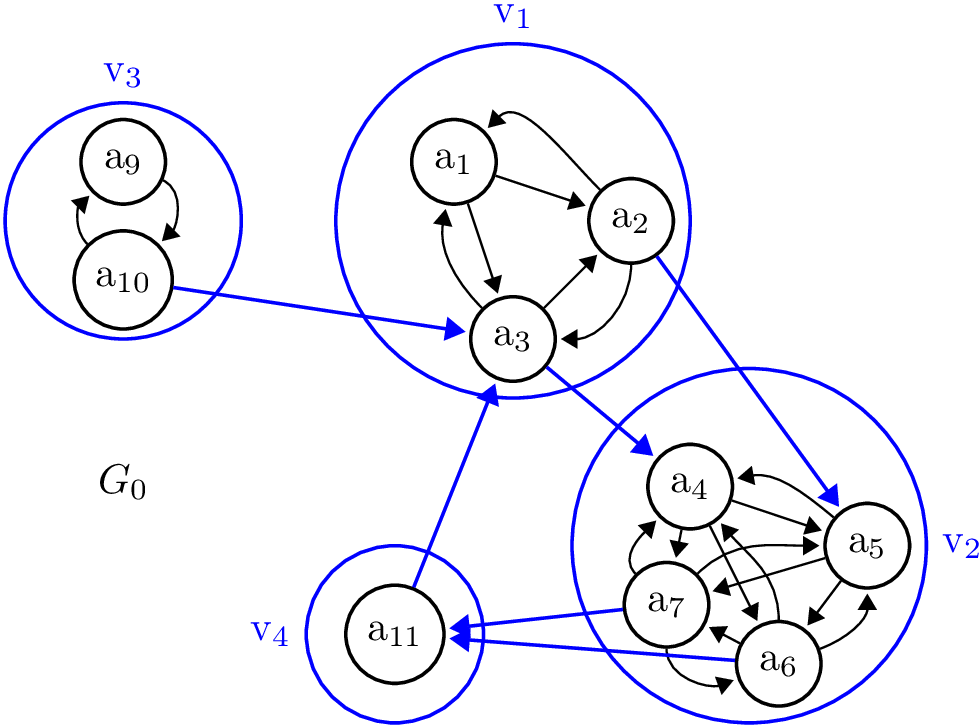
\includegraphics[scale=0.315]{Immagini/graph0.png}
    };

    \node[canvas is zy plane at x=5,draw,fill=white] at (0,0) {
        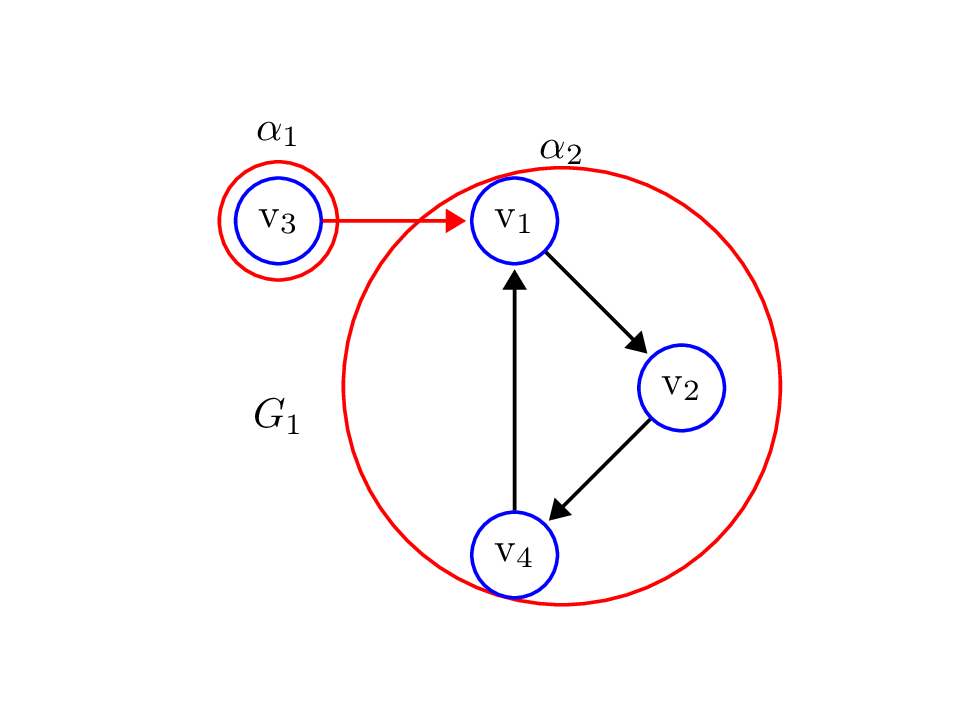
\includegraphics[scale=0.315]{Immagini/graph1.png}
    };

    \node[canvas is zy plane at x=10,draw,fill=white] at (0,0) {
        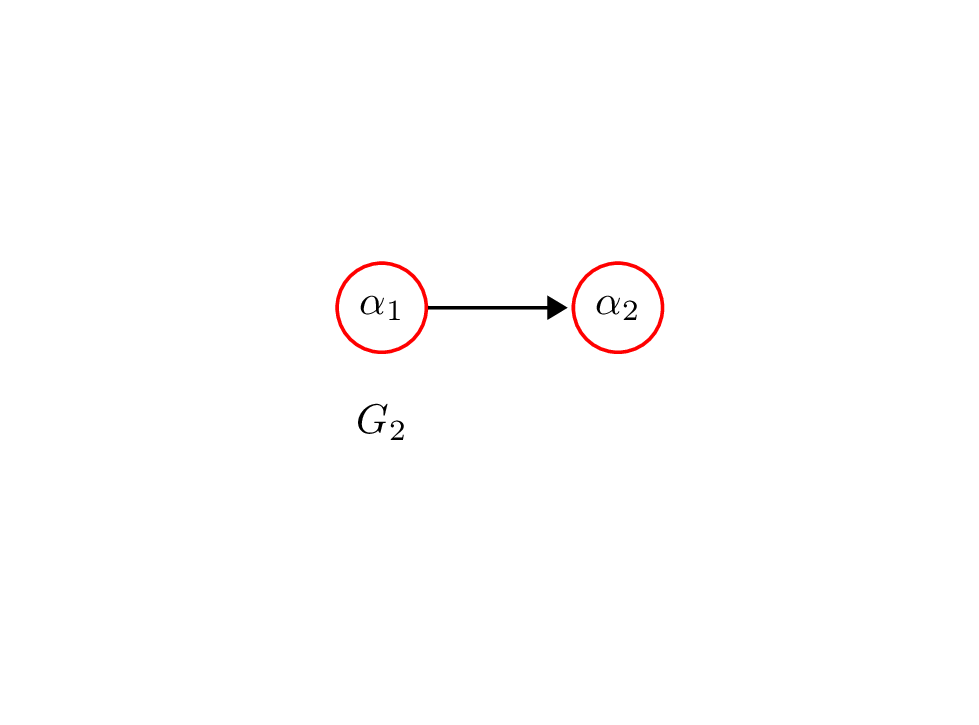
\includegraphics[scale=0.315]{Immagini/graph2.png}
    };
\end{tikzpicture}
    \caption{Esempio di grafo multi-livello}
    \label{fig:multi-level-graph-example}
\end{figure}

\newpage

\nlparagraph{Algoritmo di trasformazione naturale}\label{subsec:algoritmo-di-trasformazione-naturale}

La generica procedura algoritmica per realizzare la trasformazione naturale di un grafo standard $H = (W, F)$
preso in input in un grafo decontraibile $G = (V, E, dec_V, dec_E)$, può essere definita considerando la creazione di
supernodi e superarchi, costruendo implicitamente la funzione biiettiva $f_V: W \rightarrow V$ che realizza
l'isomorfismo tra i nodi di $H$ e i supernodi di $G$.

\begin{algorithm}[H] \floatname{algorithm}{Algoritmo}
    \begin{algorithmic}[1]
        \caption{NATURAL-TRANSFORMATION($H$)}\label{alg:natural-transformation}
        \State Sia $G = (V, E)$ un nuovo grafo decontraibile, con $V = \emptyset$ e $E = \emptyset$
        \For{$x \in W$}
            \State Sia $v$ un nuovo supernodo
            \State $v.dec \coloneqq (\emptyset, \emptyset)$
            \State $V \coloneqq V \cup \{v\}$
        \EndFor
        \For{$(x,y) \in F$}
            \State Sia $e$ un nuovo superarco
            \State $e.dec \coloneqq \emptyset$
            \State $E \coloneqq E \cup \{e\}$
        \EndFor
        \State \Return $G$
    \end{algorithmic}
\end{algorithm}

Tramite l'ausilio di strutture dati con tempi di ricerca costanti, come insiemi di hash, la complessit\`a delle
operazioni all'interno dei due cicli \`e $O(1)$,
e, di conseguenza, la complessit\`a dell'algoritmo \`e dettata dal numero di nodi e archi del grafo in input $H$,
ovvero $\mathbf{\Theta(|W| + |F|)}$.
\section{Procedure di Contrazione}\label{cap:procedure-contrazione}

In questa sezione si entrerà nel merito delle dinamiche interne alla costruzione della struttura di un grafo
multi-livello e alle sue funzioni di contrazione.
Sebbene nella Sezione~\ref{sec:algoritmi-di-enumerazione} siano già stati illustrati gli
algoritmi specifici per il riconoscimento e l'elencazione di pattern strutturali all'interno di un grafo,
nulla è stato ancora detto di come queste procedure di enumerazione debbano essere sfruttate nel contesto più
complesso del grafo multi-livello.
In particolare, si vuole dare una visione più chiara di come sia algoritmicamente
possibile realizzare una rete di collegamenti tra supernodi su più livelli attenendosi alle definizioni
fornite nella Sezione~\ref{sec:definizioni-e-proprieta-di-base} di questo capitolo, affinché si possa ottenere un tale
risultato a partire da una qualsiasi sequenza di insiemi di nodi generati dalle procedure di enumerazione,
evidenziandone complessità, problematiche e possibili soluzioni.

\subsection{Riduzione disgiunta}

Si vuole ora considerare il generico problema per cui, dato un grafo decontraibile $G = (V, E)$ e un insieme di
sottoinsiemi di nodi $Q \subseteq \mathcal{P}(V)$ che costituisce una copertura di $V$, si vuole costruire un grafo
decontraibile $G'$ che rappresenti l'informazione fornita dal raggruppamento dei nodi descritto in $Q$.
Aspetto di fondamentale importanza è che l'insieme $Q$ non costituisce necessariamente una partizione.
$Q$ potrebbe quindi essere calcolato a partire da un grafo $G$ attraverso un algoritmo di enumerazione, in modo tale
che i suoi elementi siano insiemi di nodi appartenenti ad un certo pattern strutturale.
Tuttavia, come si può immaginare, tali insiemi non sono necessariamente disgiunti: basti pensare alle cricche e i
circuiti semplici, che possono avere nodi in intersezioni di più insiemi.
Le componenti fortemente connesse invece, essendo costruite a partire da una relazione di equivalenza, sono un
valido esempio di pattern strutturale che costituisce sempre una partizione di $V$. \newline

D'ora in avanti, ci riferiremo agli elementi di una tale copertura di nodi $Q$ (non necessariamente disgiunta)
come \textbf{insiemi componenti} \newline

Per mantenere le proprietà delle contrazioni su grafi è però necessario che ad ogni nodo corrisponda ad uno ed un solo
supernodo.
La presenza dello stesso nodo in più supernodi contratti non sarebbe coerente con la teoria dei grafi
già affermata, oltre che portare ad un risultato che rischia di avere limitate applicabilità.
Si vuole quindi definire una procedura per rappresentare l'informazione fornita da $Q$ in un nuovo insieme che sia una
partizione di $V$ rappresentativa di $Q$ e, a partire da questa, costruire un grafo decontraibile $G'$.
Abbinare questa definzione generica, valida nella teoria degli insiemi, ad uno specifico algoritmo per calcolare
$Q$ a partire dalla struttura di un grafo, è il primo passo che permetterà di definire particolari funzioni di
contrazione.

\nlparagraph{Definzione}

\begin{definition}[Riduzione disgiunta]
Sia $V$ un insieme di elementi. Sia $Q \subseteq \mathcal{P}(V)$ una copertura di $V$.
Definiamo la \textbf{riduzione disgiunta} di $Q$, e la indichiamo con $\mathcal{D}(Q)$,
l'insieme di insiemi di elementi in $V$ tale per cui:
\begin{enumerate}[(i)]
    \item $\emptyset \notin \mathcal{D}(Q)$
    \item $\forall A \in \mathcal{D}(Q), \quad u, v \in A \Leftrightarrow \{C \in Q \mid u \in C\} = \{C \in Q \mid v \in C\}$
\end{enumerate}
\end{definition}

Una riduzione disgiunta di una copertura $Q$ è quindi un insieme di insiemi di nodi in $V$ tale per cui due
nodi $u$ e $v$ appartengono allo stesso insieme in $\mathcal{D}(Q)$ se e solo se sono inclusi nella stessa combinazione
di insiemi in $Q$. \newline

\begin{figure}[!h] \centering
\resizebox{!}{5.3cm}{
    \begin{tikzpicture}[state/.style ={circle, draw, color=black , fill=blue, text=white, inner sep=0cm,
    minimum size=0.1cm}]
        \node[state] (1) [label={[left,text=blue]:$v_1$}] at (-0.3, 0) {};
        \node[state] (2) [label={[left,text=blue]:$v_2$}] at (1, 0.5) {};
        \node[state] (3) [label={[left,text=blue]:$v_3$}] at (0, -0.6) {};
        \node[state] (4) [label={[right,text=blue]:$v_4$}] at (-0.4, 0.8) {};
        \node[state] (5) [label={[right,text=blue]:$v_5$}] at (0.8, 1.7) {};
        \node[state] (6) [label={[left,text=blue]:$v_6$}] at (1.9, 2.3) {};
        \node[state] (7) [label={[left,text=blue]:$v_7$}] at (4, 0) {};
        \node[state] (8) [label={[left,text=blue]:$v_8$}] at (3.2, -0.8) {};
        \node[state] (9) [label={[right,text=blue]:$v_9$}] at (3.6, -0.8) {};
        \node[state] (10) [label={[right,text=blue]:$v_{10}$}] at (2.5, 0.5) {};
        \node[state] (11) [label={[below,text=blue]:$v_{11}$}] at (4, 1.5) {};
        \node[state] (12) [label={[above,text=blue]:$v_{12}$}] at (4.5, 1.2) {};

        \node[fit={(1)(2)(3)(4)}, draw, circle, label=below:$C_1$]{};
        \node[fit={(5)(6)}, draw, circle, label=left:$C_5$]{};
        \node[fit={(7)(10)},draw, ellipse, label=right:$C_4$, minimum width = 2.7cm]{};
        \node[fit={(2)(10)},draw, ellipse, label=below:$C_3$, minimum width = 2.7cm, minimum height = 1cm]{};
        \node[fit={(7)(8)(9)(10)(11)(12)}, draw, circle, label=above:$C_2$]{};
        \node[fit={(11)(12)}, draw, circle, label=left:$C_6$]{};
        \node (Q) at (2.3, -2) {$Q$};
    \end{tikzpicture}
    \hspace{0.5cm}
    \begin{tikzpicture}[state/.style ={circle, draw, color=black , fill=blue, text=white, inner sep=0cm,
    minimum size=0.1cm}]
        \node[state] (1) [label={[left,text=blue]:$v_1$}] at (-0.3, 0) {};
        \node[state] (2) [label={[left,text=blue]:$v_2$}] at (1, 0.5) {};
        \node[state] (3) [label={[left,text=blue]:$v_3$}] at (0, -0.6) {};
        \node[state] (4) [label={[right,text=blue]:$v_4$}] at (-0.4, 0.8) {};
        \node[state] (5) [label={[right,text=blue]:$v_5$}] at (0.8, 1.7) {};
        \node[state] (6) [label={[left,text=blue]:$v_6$}] at (1.9, 2.3) {};
        \node[state] (7) [label={[left,text=blue]:$v_7$}] at (4, 0) {};
        \node[state] (8) [label={[left,text=blue]:$v_8$}] at (3.2, -0.8) {};
        \node[state] (9) [label={[right,text=blue]:$v_9$}] at (3.6, -0.8) {};
        \node[state] (10) [label={[right,text=blue]:$v_{10}$}] at (2.5, 0.5) {};
        \node[state] (11) [label={[below,text=blue]:$v_{11}$}] at (4, 1.5) {};
        \node[state] (12) [label={[above,text=blue]:$v_{12}$}] at (4.5, 1.2) {};

        \node[fit={(1)(3)(4)}, draw, ellipse]{};
        \node[fit={(5)(6)}, draw, circle]{};
        \node[fit={(2)}, draw, circle]{};
        \node[fit={(10)}, draw, circle]{};
        \node[fit={(7)}, draw, circle]{};
        \node[fit={(8)(9)}, draw, ellipse, minimum width = 2cm]{};
        \node[fit={(11)(12)}, draw, circle]{};
        \node (DQ) at (2.2, -2) {$D(Q)$};
    \end{tikzpicture}}
\caption{Esempio di riduzione disgiunta}
\label{fig:disjoint_reduction_example}
\end{figure}

L'esempio in Figura~\ref{fig:disjoint_reduction_example} fornisce una rappresentazione di una copertura $Q$ di
elementi (a sinistra) accompagnata dalla sua riduzione disgiunta $D(Q)$ (a destra).

Il nome di questa definizione deriva dal fatto che:
\begin{itemize}
    \item il risultato di questo operatore su una copertura $Q$, da solo non contiene le informazioni sufficienti a
        descrivere la copertura che lo ha originato, che potrebbero essere molteplici (ma non infinite, se si ha a che
        fare con insiemi finiti). %TODO: nota: potrebbe essere una classe di equivalenza tra coperture!!
        Da qui il termine \("\)riduzione\("\).
    \item il risultato di questo operatore su una copertura $Q$ di $V$ costituisce una partizione di $V$, come
        dimostrato in seguito, e fornisce un criterio per una suddivisione degli elementi in $V$ in insiemi disgiunti
        tra loro.
        Da qui il termine \("\)disgiunta\("\).
\end{itemize}

\begin{proposition}
Sia $V$ un insieme di elementi. Sia $Q \subseteq \mathcal{P}(V)$ una copertura di $V$.
La riduzione disgiunta di $Q$ costituisce una partizione di $V$.
\end{proposition}

\paragraph{Dimostrazione}
Si definisce la relazione $R_Q$ sull'insieme $V$ come
\begin{equation*}
    uR_{Q}v \Leftrightarrow \{C \in Q \mid u \in C\} = \{C \in Q \mid v \in C\}
\end{equation*}

Essa \`e una relazione di equivalenza, in quanto rispetta le propriet\`a di riflessivit\`a, simmetria e transitivit\`a,
che sono date dalle rispettive propriet\`a dell'uguaglianza.
Segue che l'insieme quoziente $V/R_{Q}$ deve rappresentare una partizione degli elementi in $V$.

Per il punto (ii) della definzione di $\mathcal{D}(Q)$, i suoi insiemi non vuoti rappresentano le classi di equivalenza
di $R_Q$.
Inoltre per il punto (i), l'insieme vuoto non pu\`o appartenere a $D(Q)$.
Si conclude allora $D(Q) = V/R_{Q}$, e pertanto $D(Q)$ \`e una partizione di $V$.

\nlparagraph{Definizione tramite ipergrafi}

Un \textit{ipergrafo} è una struttura simile ad un grafo non orientato dove ogni arco, detto \textit{iperarco},
anziché collegare una semplice coppia di nodi può connettere un arbitrario sottoinsieme di vertici.
Più formalmente, un ipergrafo $H$ è una coppia $(X, E)$ dove $X$ è un insieme di elementi chiamati nodi ed $E$ è
un insieme di sottoinsiemi di $X$ chiamati iperarchi.
Si consideri ora un ipergrafo non orientato $H = (X, E)$.
Notando che un iperarco non orientato $e \in E$ è a tutti gli effetti un insieme di nodi $e \subseteq V$,
si pu\`o estendere il concetto di rappresentazione disgiunta anche nel dominio degli ipergrafi.

\begin{definition}[Riduzione disgiunta di un ipergrafo]
    Dato un ipergrafo non orientato $H = (X, E)$ tale per cui $E$ \`e un ricoprimento di $X$,
    definiamo \textbf{riduzione disgiunta} di $H$ un nuovo ipergrafo non orientato $J = (W, F)$
    tale per cui $W = V$ e $F = \mathcal{D}(E)$.
\end{definition}

Si pu\`o notare, quindi, che la funzione di riduzione disgiunta pu\`o essere considerata come una
endofunzione idempotente sull'insieme degli ipergrafi non orientati.

\nlparagraph{Contrazione costruita da una partizione}

Motivo per cui la riduzione disgiunta di una copertura è certamente utile nel momento in cui si voglia
realizzare una funzione di contrazione, è che essa permette di ottenere una partizione di nodi.
La seguente ulteriore definizione permette di chiarire il passaggio che porta alla produzione in output di un grafo
decontraibile.

\begin{definition}[Contrazione costruita da una partizione]
Sia $G = (V, E)$ un grafo decontraibile, sia $P$ una partizione di $V$.
Si definisce \textbf{contrazione di $G$ costruita sulla partizione $P$} il grafo decontraibile
$G' = (\mathfrak{V}, \mathfrak{E})$ contrazione di $G$ tale per cui
    \begin{equation*}
        \{V_\alpha \mid \alpha \in \mathfrak{V}, dec_{\mathfrak{V}}(\alpha) = (V_\alpha, E_\alpha)\} = P
    \end{equation*}
\end{definition}

Dato un grafo decontraibile $G$ e una sua partizione dei nodi, quindi, è sempre possibile calcolare la sua
contrazione $G'$ contraendo nodi di $G$ in supernodi di $G'$ secondo gli insiemi descritti dalla partizione.
Si noti, infatti, che esiste una biiezione tra l'insieme delle possibili contrazioni di $G$ e l'insieme delle
partizioni di $V$ e che, pertanto, data una partizione di $V$ esiste una ed una sola contrazione di $G$ costruita
su di essa.

\nlparagraph{Algoritmo per la contrazione costruita da una riduzione disgiunta}\label{sec:make_decontractible_graph}

Entrambi i concetti esposti nel paragrafo precedente, ovvero la riduzione disgiunta di una copertura e la
contrazione costruita da una partizione, sono considerabili come elementi sufficientemente generici
per la definizione di una qualsiasi procedura di contrazione.
In particolare, il passaggio da una copertura
di nodi ad un grafo decontraibile può essere considerato come l'operazione successiva all'enumerazione degli
insiemi di nodi che costituiscono la copertura stessa. \newline

Risulta quindi utile definire un algoritmo che a partire da un grafo decontraibile $G$ e una sua copertura $Q$,
fornisca in output la contrazione di $G$ costruita sulla riduzione disgiunta di $Q$.

Una delle possibili rappresentazioni della copertura $Q$, da fornire in input a tale algoritmo, è quella un
\textit{dizionario} (talvolta anche detto ``mappa'' o ``tabella''), una struttura dati astratta che rappresenta una
collezione di coppie di elementi chiave-valore e le cui operazioni fondamentali consistono nell'inserimento e
cancellazione di coppie e ricerca di un valore mediante la sua chiave. \`E importante che in un dizionario
ad ogni chiave corrisponda al più un solo valore.
Negli pseudocodici, dato un dizionario $T$, l'operazione di ricerca di un valore associato ad una chiave $k$ verrà
indicata con $T[k]$, mentre l'operazione di inserimento di una coppia chiave-valore $(k, v)$ con $T[k] = v$.
Con $T.keys$ e $T.values$ si indicano rispettivamente l'insieme delle chiavi e l'insieme dei valori contenuti in $T$.

La copertura $Q$ è quindi data da un dizionario $T$ di dimensione $|V|$, in cui le coppie chiave-valore consistono di:
\begin{itemize}
    \item Chiave: nodo $v \in V$
    \item Valore: l'insieme di insiemi componenti $C \in Q$ tali per cui $v \in C$
\end{itemize}

Nel corso dell'algoritmo un altro dizionario $T'$ viene usato allo scopo di mappare la biiezione tra gli elementi
di $\mathcal{D}(Q)$ (quindi le classi di equivalenza di $V/R_Q$) e i supernodi di $G'$.
Aggiungendo coppie a $T'$, naturalmente al termine dell'algoritmo il dizionario $T'$ dovrà raggiungere la dimensione
$|\mathcal{D}(Q)|$. \newline

Nel ciclo a riga 3, si assegna ogni nodo del grafo decontaibile in input $G$ ad un supernodo, che esso sia
creato contestualmente o che sia il supernodo già creato corrispondente all'insieme di insiemi componenti in $v$.
Essendo che le precondizioni impongono che $T$ rappresenti una copertura di $V$, l'insieme $G.V$ a riga 3
potrebbe essere sostituito con $T.keys$.
Nel ciclo a riga 15, si assegnano gli archi di $G$ ai superarchi di $G'$. Se l'arco $(v, w)$ è interno ad un
supernodo, esso viene assegnato al suo insieme di archi. Se invece l'arco è tra collega due supernodi distinti, esso
viene assegnato al superarco corrispondente, che potrebbe essere contestualmente creato.

\begin{algorithm}[H] \floatname{algorithm}{Algoritmo}
    \caption{MAKE-DECONTRACTIBLE-GRAPH($T,G$)}\label{alg:make-decontractible-graph}
    \begin{algorithmic}[1]
        \State Sia $G' = (\mathfrak{V}, \mathfrak{E})$ un nuovo grafo decontraibile, con $\mathfrak{V} = \emptyset$
                e $\mathfrak{E} = \emptyset$
        \State Sia $T\mathcal{'}$ una nuova tabella, con insiemi di nodi come chiavi e supernodi come valori
        \For{$v\in G.V$}
            \If {$T[v]\notin T\mathcal{'}.keys$}
                \State Sia $\beta$ un nuovo supernodo con $G_{\beta}$ = $(\emptyset, \emptyset)$
                \State $\mathfrak{V}$ $\coloneqq$ $\mathfrak{V}$ $\cup$ $\{\beta\}$
                \State $T'[T[v]] \coloneqq \beta$
                \State $\alpha \coloneqq \beta$
            \Else
                \State $\alpha \coloneqq T'[T[v]]$
            \EndIf
            \State $V_{\alpha} \coloneqq V_{\alpha}$ $\cup$ $\{v\}$
            \State $v.supernode \coloneqq \alpha$
        \EndFor
        \For {$(v,w)$ in $G.E$}
            \State $\alpha \coloneqq v.supernode$
            \State $\beta \coloneqq w.supernode$
            \If {$(\alpha == \beta )$}
                \State $E_{\alpha} \coloneqq E_{\alpha} \cup \{(v,w)\}$
            \Else
                \If {$(\alpha , \beta)$ $\notin$ $\mathfrak{E}$}
                    \State $\mathfrak{E}$ $\coloneqq$ $\mathfrak{E}$ $\cup$ $\{(\alpha , \beta)\}$
                \EndIf
                \State $(\alpha , \beta).dec$ $\coloneqq$ $(\alpha , \beta).dec$ $\cup$ $\{(v, w)\}$
            \EndIf
        \EndFor
        \State \Return $G'$
    \end{algorithmic}
\end{algorithm}

In Figura~\ref{fig:make_decontractible_graph_example} sono rappresentati il grafo $G$, suddiviso in due insiemi
componenente e il corrispondente dizionario $T$ che ne rappresenta la copertura. Il dizionario $T\mathcal{'}$ \`e
rappresentato nello stato seguente all'applicazione dell'algoritmo MAKE-DECONTRACTIBLE-GRAPH con input $T$ e $G$,
contenendo come insieme di valori i supernodi ottenuti dalla contrazione di $G$.
Il risultato di MAKE-DECONTRACTIBLE-GRAPH($T$, $G$) \`e in questo caso il grafo decontraibile
$G'=(\{\alpha_1, \alpha_2, \alpha_3\}, \{(\alpha_1, \alpha_2), (\alpha_2, \alpha_3)\})$

\begin{figure}[H]
    \centering
    \begin{multicols}{3}
    \hspace{-1cm}
    \begin{tabularx}{0.8\linewidth} {
        | >{\raggedright\arraybackslash}X
        | >{\centering\arraybackslash}X | }
        \multicolumn{2}{>{\hsize=\dimexpr2\hsize+2\tabcolsep+\arrayrulewidth\relax}X}{\center$T$} \\
        \hline
        $v_1$ & $\{C_1\}$\\
        \hline
        $v_2$ & $\{C_1\}$\\
        \hline
        $v_3$ & $\{C_1, C_2\}$\\
        \hline
        $v_4$ & $\{C_2\}$\\
        \hline
        $v_5$ & $\{C_2\}$\\
        \hline
    \end{tabularx}
    \columnbreak \hspace{-1.75cm}
    \begin{tabularx}{0.8\linewidth} {
        | >{\raggedright\arraybackslash}X
        | >{\centering\arraybackslash}X | }
        \multicolumn{2}{>{\hsize=\dimexpr2\hsize+2\tabcolsep+\arrayrulewidth\relax}X}{\center$T'$} \\
        \hline
        $\{C_1\}$ & $\alpha_1$\\
        \hline
        $\{C_1, C_2\}$ & $\alpha_2$\\
        \hline
        $\{C_2\}$ & $\alpha_3$\\
        \hline
    \end{tabularx}
    \columnbreak \hspace{-1cm}
    \begin{tikzpicture}

        \node[circle, draw] (A) {$v_1$};
        \node[circle, draw] (B) [above of=A, node distance=1.4cm] {$v_2$};
        \node[circle, draw] (C) [right=0cm and 1cm of B] {$v_3$};
        \node[circle, draw] (D) [right=0cm and 1cm of C] {$v_4$};
        \node[circle, draw] (E) [below of=D, node distance=1.4cm] {$v_5$};
        \begin{pgfonlayer}{background}
            \node[blue,
            circle,
            draw,
            fit=(A)(B)(C),
            label={[align=center, black]above:{$C_1$}}] (set1) {};
        \node[red,
            circle,
            draw,
            fit=(C)(D)(E),
            label={[align=center, black]above:{$C_2$}}] (set2) {};

        \end{pgfonlayer}
        \draw[myarrow] (A) -- (B);
        \draw[myarrow] (B) -- (C);
        \draw[myarrow] (A) -- (C);
        \draw[myarrow] (C) -- (D);
        \draw[myarrow] (D) -- (E);
        \draw[myarrow] (C) -- (E);
    \end{tikzpicture}
\end{multicols}
    \vspace{-30pt}
    \caption{Esempio di tabelle $T$ e $T'$ e del corrispondente grafo decontraibile}
    \label{fig:make_decontractible_graph_example}
\end{figure}

\paragraph{Complessità}
Facendo uso di tabelle di hash per rappresentare i dizionari $T$ e $T'$, l'algoritmo mantiene una complessit\`a
temporale di $O(|V| + |E|)$.
Si noti infatti che:
\begin{itemize}
    \item Il primo ciclo for scorre tutti i nodi in $V$.
    Esso inizializza il dizionario $T'$, definisce i supernodi di $G'$ e assegna loro i nodi in $V$.
    La complessità del ciclo è $O(|V|)$, infatti il controllo a riga 3 ha complessità costante,
    così come le ricerca in $T$ e $T'$ alle righe 7 e 10.
    \item Il secondo ciclo for scorre tutti gli archi in $E$.
    Esso assegna gli archi di $G$ ai grafi dei supernodi di $G'$ o ai superarchi di $G'$ a seconda dei supernodi
    di appartenenza dei nodi che li compongono, ottenibili in tempo $O(1)$ in quanto precedentemente calcolati nel
    primo ciclo for. La complessit\`a del ciclo \`e $O(|E|)$.
\end{itemize}

\subsection{Algoritmi di contrazione}\label{sec:algoritmi-di-contrazione}

In questa sezione illustriamo brevemente come a partire dagli algoritmi di enumerazione di sottoinsiemi descritti
e dall'algoritmo per la contrazione costruita da una rappresentazione disgiunta, \`e quindi possibile costruire
delle procedure complete che rappresentino delle funzioni di contrazione.

\nlparagraph{Procedure per la gestione dei dizionari}\label{subsec:procedure-per-la-gestione-deli-dizionari}

Come si pu\`o notare dallo pseudo-codice dagli algoritmi di enumerazione descritti nel
Capitolo~\ref{ch:algoritmi-di-enumerazione}, ciascuno di essi provvede a fornire in output una sequenza di
sottoinsiemi di nodi che rispettino il pattern strutturale individuato.
Allo scopo di costruire una funzione di contrazione, \`e però necessario che tali insiemi siano usati per definire
una copertura di nodi rappresentata attraverso un dizionario $T$, come descritto nella sezione precedente.
Per questo motivo si propongono una serie di procedure che permettano di inizializzare, aggiungere e rimuovere
sottoinsiemi da un dizionario $T$, affinché queste possano essere usate come integrazione per fornire un
adattamento dello pseudo-codice originale degli algoritmi di enumerazione presentati. \newline

In particolare, come riga iniziale di ciascuno di questi algoritmi, può essere aggiunta la seguente procedura per
l'inizializzazione del dizionario $T$.

\begin{algorithm}[H]
    \caption{INITIALIZE-TABLE($V$)}\label{alg:init-table}
    \begin{algorithmic}[1]
        \State Let $T$ be a new table
        \For{$v \in V$}
            \State $T[v] \coloneqq \emptyset$
        \EndFor
        \State return $T$
    \end{algorithmic}
\end{algorithm}

L'operazione di fornire in output un insieme componente potrebbe essere invece sostituita in ciascun algoritmo
con la seguente procedura per l'aggiunta di un insieme $C$ all'insieme di insiemi componente tracciati da $T$. \newline

\begin{algorithm}[H] \floatname{algorithm}{Algoritmo}
    \caption{ADD-COMPONENT-SET($T$, $C$)}\label{alg:add-subset}
    \begin{algorithmic}[1]
        \For{$v\in C$}
            \State $T[v]:=T[v] \cup \{C\}$
            \State $T.modified:=T.modified \cup \{v\}$
        \EndFor
    \end{algorithmic}
\end{algorithm}

Per completezza si fornisce anche la procedura per la rimozione di un insieme $C$ da $T$.

\begin{algorithm}[H]
    \caption{REMOVE-SUBSET($T$, $C$)}\label{alg:rem-subset}
    \begin{algorithmic}[1]
        \For{$v\in C$}
            \State $T[v]:=T[v] \setminus \{C\}$
            \State $T.modified:=T.modified \cup \{v\}$
        \EndFor
    \end{algorithmic}
\end{algorithm}

Nel caso in cui si avesse a che fare con procedure di enumerazione che forniscono in output insiemi di nodi che non
necessariamente forniscono una copertura di tutti i nodi del grafo (come nel caso dell'algoritmo di enumerazione
dei circuiti semplici), la seguente procedure può essere utilizzata al termine dell'enumerazione per aggiungere
ciascun nodo rimasto escluso dalla copertura a un insieme componente singoletto. Come evidente dallo
pseudocodice, tale procedura manterrebbe una complessit\`a temporale di $O(|V|)$, con |V| il numero di nodi del grafo
decontraibile da contrarre.

\begin{algorithm}[H] \floatname{algorithm}{Algoritmo}
    \caption{ADD-SINGLETONS($T$)}\label{alg:add-singletons}
    \begin{algorithmic}[1]
        \For{$v \in T.keys$}
            \If{$T[v] == \emptyset$}
                \State $T[v] := \{v\}$
            \EndIf
        \EndFor
    \end{algorithmic}
\end{algorithm}

Si pu\`o notare che le procedure di aggiunta e rimozione di un sottoinsieme $C$ da $T$ prevedono il tracciamento
dei particolari nodi corrispondenti a record di $T$ modificati, attraverso l'utilizzo di un insieme associato
alla tabella e indicato come $T_{modified}$.
Sebbene non sia necessario per le procedure di contrazione, questo risulterà utile per rendere le procedure
applicabili anche nelle procedure di aggiornamento dinamico al grafo contratto, come verrà trattato nel capitolo~\ref{}.
L'insieme $T_{modified}$ permetterà, infatti, di evitare di scorrere l'intero dizionario $T$ nel momento in cui il
grafo contratto già costruito dovrà essere aggiornato in accordo alle modifiche agli insiemi componente tracciati
da $T$. \newline

\nlparagraph{Aggiunta di un sottoinsieme massimale}

Sebbene alcuni algoritmi di enumerazione possano già fornire in output sottoinsiemi di nodi tra loro massimali,
come nel caso dell'algoritmo di enumerazione delle componenti fortemente connesse e delle cricche massimali,
in generale non è garantito che ciò avvenga, come nel caso dell'algoritmo di enumerazione dei circuiti semplici.
Qualora sia necessario adattare una funzione di contrazione affinché questa sia basata sui soli insiemi di nodi
massimali forniti da un algoritmo di enumerazione, la procedura descritta di seguito può essere utilizzata in
sostituzione della normale procedura ADD-COMPONENT-SET.
Infatti, questa procedura permette controllare contestualmente alla sua aggiunta a $T$ se un dato sottoinsieme $C$ di
nodi sia massimale rispetto agli altri insiemi già tracciati in $T$ e, se si, individuare quali eventuali sottoinsiemi
in $T$ siano inclusi in $C$, affinché possano essere rimossi.

\begin{algorithm}[H]
    \caption{ADD-MAXIMAL-SUBSET($T$, $C$)}\label{alg:add-maximal-subset}
    \begin{algorithmic}[1]
        \If{$\bigcap_{v \in C}T[v] == \emptyset$}
            \State $Q :=$ FIND-SUBSETS($T$, $C$)
            \For {$S \in Q$}
                \State REMOVE-SUBSET($T$, $S$)
            \EndFor
            \State ADD-SUBSET($T$, $C$)
        \EndIf
    \end{algorithmic}
\end{algorithm}
\begin{algorithm}[H] \floatname{algorithm}{Algoritmo}
    \caption{FIND-SUBSETS($T$, $C$)}\label{alg:find-subsets}
    \begin{algorithmic}[1]
        \State Sia $T_c$ una nuova tabella per contare le occorrenze dei sottoinsiemi
        \For{$v \in C$}
            \For{$S \in T[v]$}
                \State $T_c[S] := T_c[S] + 1$
            \EndFor
        \EndFor
        \State $Q := \emptyset$
        \For {$S \in T_c$}
            \If{$T_c[S] == |C|$}
                \State $Q := Q \cup \{S\}$
            \EndIf
        \EndFor
        \State \Return $Q$
    \end{algorithmic}
\end{algorithm}

In particolare, l'algoritmo ADD-MAXIMAL-COMPONENT-SET provvede innanzitutto a verificare a riga 1 che l'insieme $C$ non
sia gi\`a incluso in un altro insieme presente tra gli insiemi di $T$, ovvero che non sia certamente
massimale.
Questo viene verificato controllando se tutti i nodi in $C$ condividano l'appartenenza ad uno o pi\`u insiemi gi\`a
presenti. \newline
Se l'insieme $C$ \`e massimale rispetto ai nodi trovati, succesivamente l'algoritmo provvede ad individuare
gli eventuali insiemi presenti in $T$ che siano sottoinsiemi di $C$ attraverso la procedura FIND-SUBSETS.
Essa conteggia il numero di volte che ciascun sottoinsieme appare tra i nodi di $C$ rispetto al dizionario $T$.
Un conteggio pari alla cardinalit\`a dell'insieme stesso testimonia che tutti i suoi nodi sono presenti in $C$.

\paragraph{Complessit\`a}
Con l'utilizzo di insiemi basati su hash, in cui la complessit\`a per verificare l'appartenenza ad un insieme \`e
$O(1)$, la complessit\`a della procedura di ADD-MAXIMAL-SUBSET risulta essere $O(|C| \cdot c_{max})$ nel caso peggiore,
dove $|C|$ \`e la cardinalit\`a dell'insieme $C$ in input e $c_{max}$ \`e l'upper bound del numero di sottoinsiemi
massimali già tracciati dalla tabella $T$, che risulta essere massimo quando la cardinalit\`a di questi insiemi
\`e pari alla met\`a del numero di nodi del grafo $G = (V, E)$ che si sta contraendo.
Si noti che la complessit\`a apportata da $c_{max}$ non pu\`o mai essere
superiore all' esponenziale, in quanto, in generale, il numero massimo di insiemi massimali che possono essere
individuati in un insieme di $n$ elementi rimarr\`a sempre inferiore al numero di tutti i possibili sottoinsiemi,
che è $2^n$.
Sebbene il termine $c_{max}$ possa essere considerato come un $O(2^n)$ nel calcolo della complessit\`a (con $n = |V|$
il numero di nodi del grafo), esso pu\`o essere calcolato in modo pi\`u preciso come segue:

\begin{equation*}
    c_{max} \quad = \quad \binom{n}{\lfloor \frac{n}{2} \rfloor} = \frac{n\cdot(n-1)\cdot\ldots\cdot(n/2)}{\frac{n}{2}!}
\end{equation*}

La complessit\`a della procedura pu\`o essere calcolata notando che l'intersezione nel controllo a riga 1 pu\`o
impiegare al pi\`u $O((|C|-1) \cdot max_{v \in C}\{|T[v]|\})$.
Tuttavia, eseguendo le intersezioni a partire dall'insieme $T[v]$ pi\`u piccolo, individuato in tempo lineare a
$|C|$, la complessit\`a pu\`o essere ridotta a $O((|C|-1) \cdot min_{v \in C}\{|T[v]|\})$.
In ogni caso, questa complessit\`a pu\`o essere riscritta come $O(|C| \cdot c_{max})$, considerando il caso peggiore
in cui tutti i nodi in $C$ appartengono agli insiemi costruiti tramite unione tra i possibili sottoinsiemi massimali
tra i restanti $|V|-|C|$ nodi del grafo e $C$, tutti di egual cardinalit\`a.
Inoltre la procedura FIND-SUBSETS impiega anch'essa al pi\`u $O(|C| \cdot c_{max})$ tempo,
in quanto il ciclo for a riga 2 scorre tutti i nodi in $C$, mentre il ciclo for a riga 3 scorre tutti i
sottoinsiemi massimali presenti in $T$ per ogni nodo in $C$, che sono al pi\`u pari a tutti i sottoinsiemi massmali
ottenibili a partire dai restanti $|V|-1$ nodi del grafo.
Inoltre il ciclo for a riga 8 scorre tutti i sottoinsiemi massimali trovati, che sono al pi\`u pari a $c_{max} - 1$,
considerato che l'insieme $C$ deve essere anch'esso massimale.

\nlparagraph{Procedure complete di contrazione}

Forniamo ora una descrizione della struttura di un algoritmo generico che rappresenti la procedura completa di
contrazione di un grafo decontraibile $G$, ovvero che permetta di realizzare una funzione di contrazione $f_C$
che possa essere usata nella definzione di un grafo multilivello.

Esso pu\`o essere costituito dalle seguenti fasi:
\begin{enumerate}
    \item Fase di pre-elaborazione (opzionale) \\
    Dato il grafo iniziale $G$, si produce un nuovo grafo $H$ adatto ad essere fornito in input all'algoritmo
    della fase successiva.
    Questo potrebbe essere utile allo scopo di adattare il grafo all'algoritmo, migliorare le performance o
    costruire un nuovo grafo che rappresenti particolari relazioni tra i nodi del grafo originale oltre alla
    semplice adiacienza.
    \item Fase di enumerazione dei sottoinsiemi \\
    Nel grafo $H$ vengono riconosciuti i pattern strutturali dallo specifico algoritmo di enumerazione e tracciati
    sotto forma di insiemi componenti composti dai nodi che fanno parte di tali pattern.
    Il riultato \`e la mappatura $T$ tra i nodi del grafo $H$ e l'insieme dei sottoinsiemi di cui fanno parte.
    \item Fase di contrazione \\
    Viene restituita la contrazione di $G$ costruita sulla rappresentazione digiunta dei sottoinsimi individuati,
    secondo la logica dell'algoritmo MAKE-CONTRACTIBLE-GRAPH\@.
\end{enumerate}

\begin{algorithm}[H]
    \caption{GENERIC-CONTRACTION($G$)}\label{alg:generic-contraction}
    \begin{algorithmic}[1]
        \State Let $H$ be a graph obtained from $G$ by a preprocessing procedure
        \State Let $T$ be a table obtained from $H$ by a generic subset enumerating algorithm
        \State $J$ = MAKE-CONTRACTIBLE-GRAPH($T$, $G$)
        \State return $J$
    \end{algorithmic}
\end{algorithm}

Gli algoritmi di contrazione relativi ai problemi di enumerazione trattati potrebbero seguire la struttura sopra
descritta nei seguenti modi:
\begin{itemize}
    \item Per la contrazione per componenti fortemente connesse la fase di preprocessing potrebbe essere
    essere saltata, in quanto l'algoritmo di Kosaraju-Sharir e la sua versione adattata non necessitano di alcuna
    modifica al grafo orientato in input.
    \item Per la contrazione per cricche può essere utilizzata una fase di preprocessing per la costruzione
    della relativa versione non orientata di un grafo, che potrebbe sostituire tutti gli archi orientati con
    archi non orientati, oppure che potrebbe mantenere un arco non orientato solo per quelle coppie di nodi
    mutualmente adiacenti.
    La fase di enumerazione può essere realizzata dalla versione adattata dell'algoritmo di Bron-Kerbosch.
    \item Per la contrazione per circuiti semplici pu\`o essere utilizzata una fase di preprocessing per
    l'eliminazione di tutti gli archi tra nodi che non facciano parte delle stesse componenti fortemente connesse
    allo scopo di migliorare le performance della fase di enumerazone che può essere realizzata dall'algoritmo
    di Johnson nella sua versione adattata.
\end{itemize}






